\section{ The SABR Model} \label{SABR_model}
In this Chapter, we will first introduce the SABR model
 and explain how to determine the forward rate and 
 volatility using this model. We will then focus on 
 calculating implied volatility and pricing European 
 options with the SABR model. Finally, the Chapter 
 will discuss methods for estimating the parameters 
 of the SABR model.
\\\\
The SABR (Stochastic Alpha, Beta, Rho) 
model represents a significant advancement in financial modeling, 
effectively addressing the notable limitations of traditional methods
like the Black-Scholes model, which assumes 
constant volatility. Developed in 2002 by Patrick Hagan, Deep Kumar, 
Andrew Lesniewski, and Diana Woodward, the SABR model is highly respected for 
its ability to manage the dynamic and unpredictable nature of market 
volatility.
\\\\
As a two-factor model, the SABR framework models both the forward rate 
(or asset price) and its volatility as a stochastic processes. This approach 
is vital as it incorporates a stochastic behavior in volatility, significantly 
improving the model's ability to capture the true, skewed, and heavy-tailed 
nature of financial market data. By allowing for volatility fluctuations, 
the SABR model provides a flexible and realistic framework for pricing 
derivatives, proving especially useful for options with long maturities where 
the assumption of constant volatility falls short \cite{Smile}.
\subsection{Specification For The SABR Model}
The main different between the SABR model and the 
Black-Scholes model is the assumptions regrading the 
volatility, as mentioned earlier. In the Black-Scholes 
model the volatility is a assumed to be constant and 
in the SABR model the volatility evolves as a function
of time, t, the strike price, K, and the current
forward price, $F_t$. Futhermore the volatility itself
is random. So we chose the unknown coefficient $C(t,*)$
to be $\hat{\alpha} \hat{F}^{\beta}$ \cite{Smile}, where the 
"volatility" $\hat{\alpha}$ is a stochastic process itself. 
The extra randomness is scaled thought the inclusion 
of a "volatility of volatility" parameter $\nu$.
\\\\
Now we will formulate the SABR model mathematically. 
The SABR model consists of a dynamic for the forward price
and one for the volatility, since the SABR model is a 
two-factor model. The SABR model also formulate the 
how the two process is correlated. 
\begin{align}
    d \hat{F_t} &= 
    \hat{\alpha}_t \hat{F}_t^\beta dW_t^1, \quad \quad \hat{F}(0)=f   \label{f_dyn}\\
    d\hat{\alpha}_t &= \nu \hat{\alpha}_t dW_t^2, \quad \quad \hat{\alpha}(0)=\alpha \label{sigma_dyn}
\end{align}
where $W_t^{1}$ and $W_t^{2}$ are two correlated Wiener 
process and it is assumed that \cite{Smile}.
\begin{align}
    dW_t^{1}dW_t^{2}=\rho dt
\end{align}
So we have that 
parameters in the SABR model is as follows, $\alpha$ represents the initial volatility level
, $\nu$ represents the volatility of volatility, or the rate at which volatility itself changes
, $\beta$ represents the elasticity of the volatility; a common practice is to fix beta based on the underlying asset 
and as mentioned $\rho$ is the correlations between the 
two Wiener process, the asset price and its volatility. 
\\\\
So the SABR model is characterized by the stochastic process $\alpha_t$,
the parameter $\beta$, and the correlation coefficient $\rho$,
which is also reflected in its name - Stochastic Alpha Beta Rho.
In a specific variant of the SABR model, 
by setting $\beta = 1 $ and $\nu = 0$, the model reverts 
to the classic Black-Scholes framework. 
This configuration leads to a constant volatility, 
denoted $\alpha_0 $, 
and a forward process where returns follow a 
normal distribution with a mean of zero and a standard 
deviation of $\alpha_0 \sqrt{t}$. So now the SABR model
has been introduced and the analysis will continuing forward 
on how to price a swaption using the SABR model to determine the implied
volatility \cite{Smile}.
\subsection{Simulation The SABR Model}
In this Section a short view on how the process for the forward price and the volatility develops over time will be covered. 
To provide the intuition on how the dynamic listed in \autoref{f_dyn} and \autoref{sigma_dyn} behave, the dynamics is simulated ten times
for some chosen parameters is listed in \autoref{tab:parameters_sim_sabr}. 
The simulated paths is illustrated in \autoref{fig:sim_f_and_sigma} below. 
From \autoref{fig:sim_f_and_sigma} we see that the dynamics are driven by the randomness in the Wiener process and 
it develops from the initial value of the forward price and volatility.
\\
\begin{table}[H]
    \centering
    \begin{tabular}{ccc}
      \toprule
      \textbf{Parameter} & \textbf{Parameter explanation} & \textbf{Value} \\
      \midrule
      \rowcolor{lightgray!40}  $F_0$ & Initial forward rate or asset price & 100 \\
      $\alpha_0$ & Initial volatility  & 0.2 \\
      \rowcolor{lightgray!40}  $\beta$ & Elasticity parameter & 0.5 \\
      $\nu$ & Volatility of the volatility parameter & 0.25 \\
      \rowcolor{lightgray!40} $\rho$ & Correlation between the asset price and its volatility & -0.4 \\
      \bottomrule
    \end{tabular}
    \caption{Summary of parameters used for simulating the SABR model}
    \label{tab:parameters_sim_sabr}
\end{table}
\noindent

\begin{figure}[H]
    \centering
    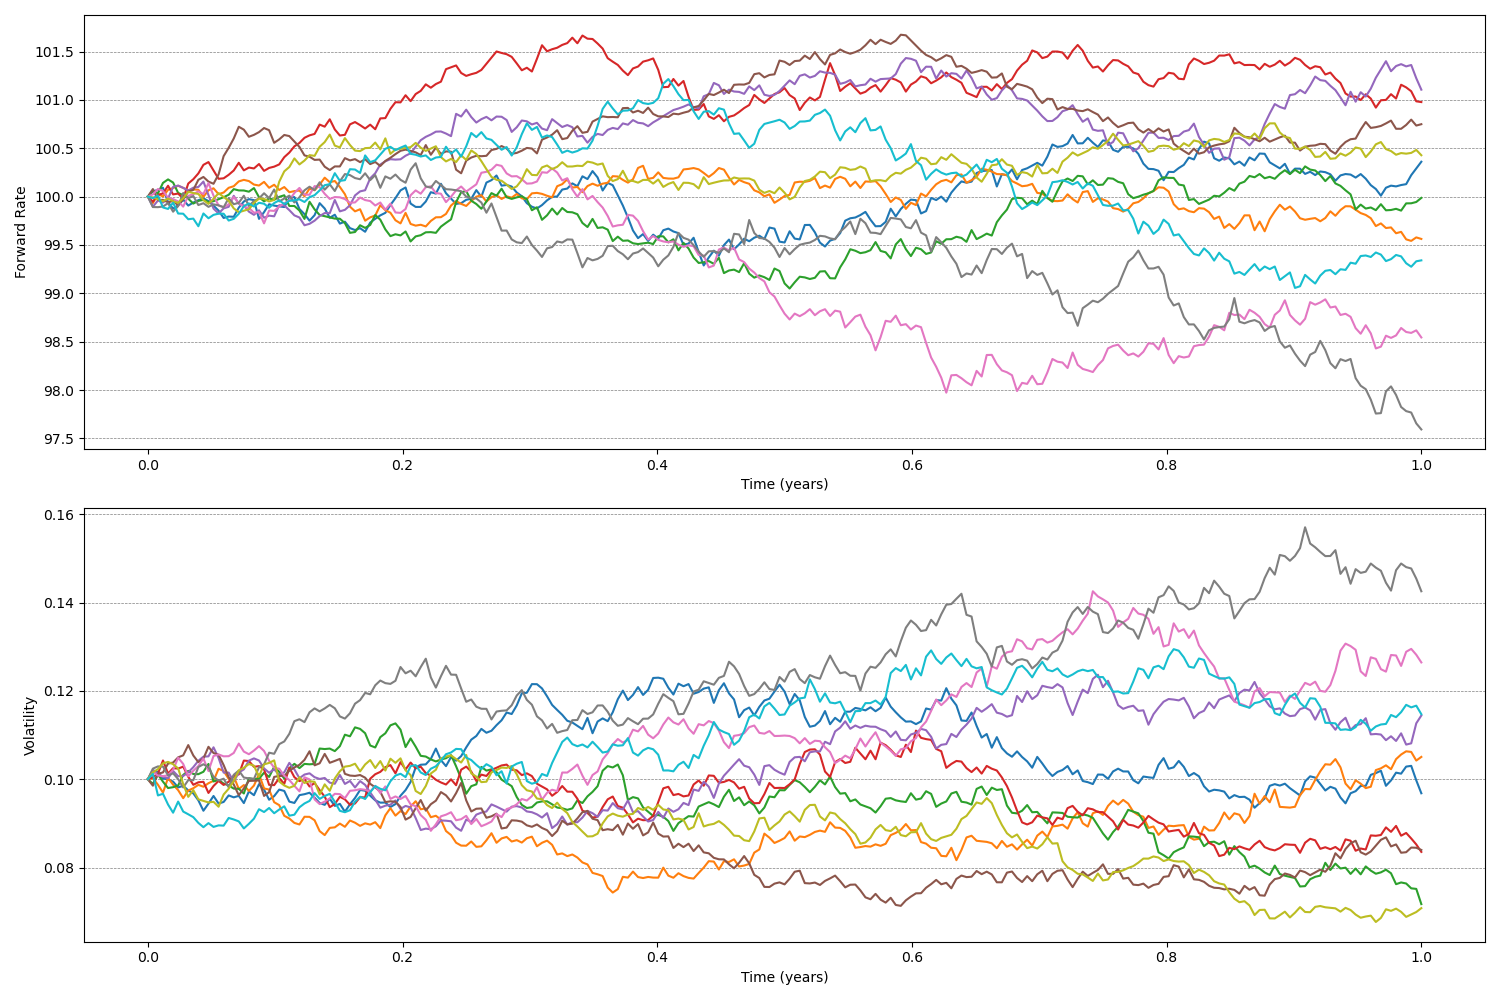
\includegraphics[width=1.\textwidth]{/Users/nannaingemannohrt/Desktop/master_thesis/main/plots/sim_f_and_sigma.png}
    \caption{Ten simulated paths for the forward rate and the volatility in the SABR model.}
    \label{fig:sim_f_and_sigma}
\end{figure}
\noindent
\subsection{SABR Implied Volatility and Option Prices}
Before we are able to move forward with the analysis,
we need to formulate how to determine implied volatility in the SABR model. 
But these calculations are out of the scope for this analysis,
so we will use the formula in the paper Managing Smile Risk 
of Hagen (2002) \cite{Smile}. The paper states that
under the SABR model, the prices of European options 
is given by Black formula in \autoref{sabr1} to \autoref{sabr3}
below
\begin{align}
    V_{\text{call}} &= D(t_{\text{set}})fN(d_1) - KN(d_2)  \label{sabr1}\\
    V_{\text{put}} &= V_{\text{call}} + D(t_{\text{set}})[K - f] \label{sabr2}
\end{align}
with
\begin{equation}
    d_{1,2} = \frac{\log \frac{f}{K} \pm \frac{1}{2}\sigma_B^2 t_{\text{ex}}}{\sigma_B \sqrt{t_{\text{ex}}}}
     \label{sabr3}
\end{equation}
here $t_{\text{set}}$ is the settlement date and $t_{\text{ex}}$ os the exercise date and 
the implied volatility $\sigma_B(f, K)$ is given by
\begin{equation}
    \sigma_B(K, f) = \frac{\alpha}{(fK)^{(1-\beta)/2}} \left\{ 1 + \frac{(1-\beta)^2}{24} \log^2 \frac{f}{K} + \frac{(1-\beta)^4}{1920} \log^4 \frac{f}{K} + \ldots \right\} \left( \frac{z}{x(z)} \right).
    \label{sigma_B}
\end{equation}
where
\begin{align}
    z &= \frac{\nu}{\alpha}(fK)^{(1-\beta)/2} \log \frac{f}{K}, \\
\end{align}
and x(z) is defined by
\begin{align}
    x(z) &= \log \left\{ \frac{\sqrt{1-2\rho z + z^2} + z - \rho}{1 - \rho} \right\}.
\end{align}
For the special case of at-the-money (ATM) options, options strike at $K = f$, this formula reduces to
\begin{equation}
    \sigma_{ATM} = \sigma_B(f, f) = \frac{\alpha}{f^{1-\beta}} \left\{ 1 + \left( \frac{(1-\beta)^2}{24} \frac{\alpha^2}{f^{2-2\beta}} + \frac{\rho \beta \nu}{4} \frac{\alpha}{f^{1-\beta}} + \frac{2-3\rho^2}{24} \nu^2 \right) t_{\text{ex}} + \ldots \right\}.
    \label{sigma_ff}
\end{equation}
\\
So we have that the parameters $\alpha, \beta, \nu$ and $\rho$  in the SABR model is estimated and the implied volatility $\sigma_B$
is a function of the forward price and the strike. Now that we have a simplified formula for the implied 
volatility from the SABR model, we can start analyzing 
how the model works. We will do this by continuing our
analysis with investigating how the different parameters 
affects implied volatility in the SABR model. 

